\documentclass[10pt,onecolumn]{article}
\usepackage{times}

\usepackage[boxed, linesnumbered]{algorithm2e}
% boxed: to have algorithms enclosed in a box
% linesnumbered: lines of the algorithms are numbered
\usepackage{graphicx}

\baselineskip 12pt
\textheight 9in
\textwidth 6.5in
\oddsidemargin 0in
\topmargin 0in
\headheight 0in
\headsep 0in

\begin{document}

\title{ZooKeeper's atomic broadcast protocol: Theory and practice}
\author{}
\date{}
\maketitle

\section{Introduction} \label{sec:intro}
Figure \S\ref{fig:paxos_run} illustrates a problem we found with Paxos under our requirements. It shows a run with three distinct proposers that violates our requirement for the order of generated state changes. Proposer P1 executes Phase 1 for sequence numbers 27 and 28. It proposes values A and B for sequence numbers 27 and 28, respectively, in Phase 2 with ballot number 1. Both proposals are accepted only by acceptor A1. Proposer P2 executes Phase 1 against acceptors A2 and A3, and end up proposing C in Phase 2 to sequence number 27 with ballot number 2. Finally, proposer P3, executes Phase 1 and 2, and is able to have a quorum of acceptors choosing C for sequence number 27, B for sequence number 28, and D for 29.

\begin{figure}[h]
\begin{center}
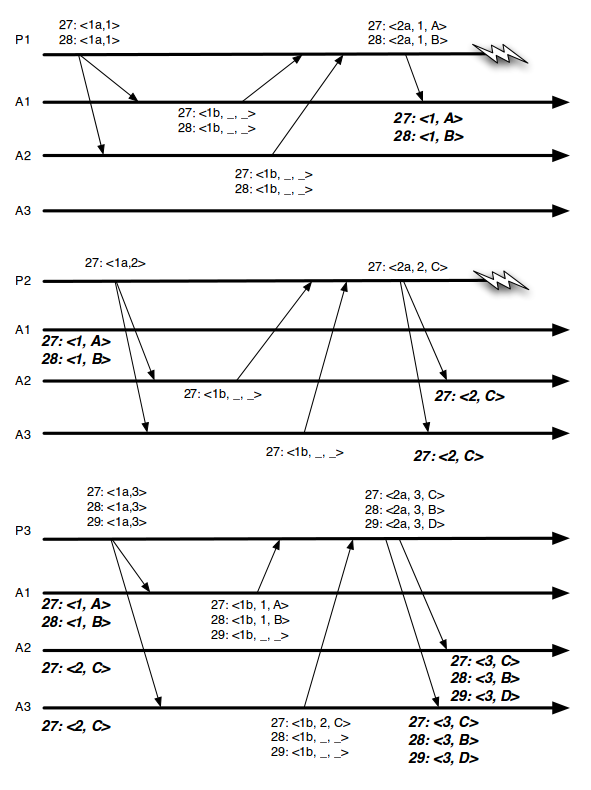
\includegraphics[height=13cm]{paxos_run.png}
\end{center}
\caption{Paxos run}
\label{fig:paxos_run}
\end{figure}

\section{Background} \label{sec:background}
\subsection{Paxos and design decisions for Zab}
Two important requirements for Zab are handling multiple outstanding client operations and efficient recovery from crashes. An outstanding transaction is one that has been proposed but not yet delivered. For high-performance, it is important that ZooKeeper can handle multiple outstanding state changes requested by the client and that a prefix of operations submitted concurrently are committed according to FIFO order.

The original Paxos protocol does not enable multiple outstanding transactions. Paxos does not require FIFO channels for communication, so it tolerates message loss and reordering. If two outstanding transactions have an order dependency, then Paxos cannot have multiple outstanding transactions because FIFO order is not guaranteed.

\subsection{Expected properties} \label{sec:property}
\emph{transactions} are state changes that the primary propagates ("broadcast") to the ensemble, and are represented by a pair $ \langle v,z \rangle$, where $v$ is the new state and $z$ is an identifier called \emph{zxid}. Transactions are first \emph{proposed} to a process by the primary, then \emph{delivered} ("committed") at a process upon a specific call to a delivery method.

\section{Atomic broadcast protocol} \label{sec:protocol}
The leader peer coordinates the phases together with the followers, and there should be at most one leader peer in Phase 3 at a time, which is also the primary process to broadcast messages. In other words, the primary is always the leader. Phases 1 and 2 are important for bringing the ensemble to a mutually consistent state, specially when recovering from crashes. They constitute the recovery part of the protocol and are critical to guarantee order of transactions while allowing multiple outstanding transactions. If crashes do not occur, peers stay indefinitely in Phase 3 participating in broadcasts, similar to the two phase commit protocol. 

ZooKeeper clients are applications that use ZooKeeper services by connecting to at least one server in the ensemble. The client submits operations to the connected server, and if this operation was submitted to a follower, it is forwarded to the leader peer. If a leader receives the operation request, then it executes and propagates the state change to its followers. Read requests from the client are directly served by any ZooKeeper server.

In Zab, transaction identifiers (zxid) are crucial for implementing total order properties. The zxid $z$ of a transaction $\langle v, z \rangle$ is a pair $\langle e, c \rangle$, where $e$ is the epoch number of the primary of the primary $p_e$ that generated the transaction $\langle v,z \rangle$, and $c$ is an integer acting as a counter. The notation $z.\mathbf{epoch}$ means $e$, and $z.\mathbf{counter} = c$. The counter c is incremented every time a new transaction is introduced by the primary. When a new epoch starts - a new leader becomes active - $c$ is set to zero and $e$ is incremented from what was known to be the previous epoch. Since both $e$ and $c$ are increasing, transactions can be ordered by their zxid.

There are four variables that constitute the persistent state of a peer, which are used during the recovery part of the protocol:
\begin{itemize}
    \item $\mathbf{history}:$ a log of transactions proposals accepted;
    \item $\mathbf{acceptedEpoch}:$ the epoch number of the last NEWEPOCH message accepted;
    \item $\mathbf{currentEpoch}:$ the epoch number of the last NEWELEADER message accepted;
    \item $\mathbf{lastZxid}:$ zxid of the last proposal in the history;
\end{itemize}

\subsection{Phases of the protocol} \label{sec:phases}
The four phases of the Zab protocol are described next.

\textbf{Phase 1: Discovery} In this phase, followers communicate with their prospective leader, so that the leader gathers information about the most recent transactions that its followers accepted. The purpose of this phase is to \textit{discover} the most updated sequence of accepted transactions among a quorum, and to establish a new epoch so that previous leaders cannot commit new proposals.
The complete description of this phase is described in Algorithm \S\ref{alg:phase1}.

% \usepackage{algorithmicx}
% \usepackage[]{algorithm}
% \usepackage{algpseudocode}
%
% \algnewcommand\algorithmicupon{\textbf{upon}}
% \algdef{SE}{Event}{EndEvent}[1]{\algorithmicupon\ #1\ \algorithmicdo}{\algorithmicend\ \algorithmicupon}
% %\algdef{<start>}{<end>}[<startparamcount>]{<start text>}[<endparamcount>]{<end text>}
%
% \begin{algorithm}[H]
% \caption{Zab Phase 1: Discovery.}
% \label{alg:phase1}
% \begin{algorithmic}[1]
%   \Event{receiving FOLLOWERINFO($e$) messages from a quorum $Q$ of connected followers}
%     \State Make epoch number $e'$ such that $e' > e$ for all $e$ received through FOLLOWERINFO($e$)
%   \EndEvent
% \end{algorithmic}
% \end{algorithm}

\begin{algorithm}[H]
  \SetAlgoNoLine % Doesn't print vertical lines
  \textit{\underline{Leader L:}} \\
  \textbf{upon} receiving FOLLOWERINFO($e$) messages from a quorum $Q$ of connected followers \textbf{do} \\
    \Indp % indents plus
    Make epoch number $e'$ such that $e' > e$ for all $e$ received through FOLLOWERINFO($e$) \\
    Propose NEWEPOCH($e'$) to all followers in $Q$ \\
  \Indm
  \textbf{end} \\
  \textbf{upon} receiving ACKEPOCH from all followers in $Q$ \textbf{do} \\
    \Indp
    Find the follower $f$ in $Q$ such that for all $f' \in Q \ \backslash \ \{f\}$: \\
      \Indp
      either $f'.\mathbf{currentEpoch} < f.\mathbf{currentEpoch}$ \\
      or $(f'.\mathbf{currentEpoch} = f.\mathbf{currentEpoch}) \wedge (f'.\mathbf{lastZxid} \preceq_{z} f.\mathbf{lastZxid})$ \\
    \Indm
    $L.\mathbf{history} \gets f.\mathbf{history}$ \quad // stored to non-volatile memory \\
    \textbf{goto} Phase 2 \\
  \Indm
  \textbf{end}
\caption{Zab Phase 1: Discovery.}
\label{alg:phase1}
\end{algorithm}

\textbf{Phase 2: Synchronization} The Synchronization phase concludes the recovery part of the protocol. The leader communicates with the followers, proposing transactions from its history. Followers acknowledge the proposals if their own history is behind the leader's history. When the leader sees acknowledgments from a quorum, it issues a commit message to them. At that point, the leader is said to be \textit{established}, and not anymore prospective.

\begin{algorithm}[H]
  \SetAlgoNoLine
  \textit{\underline{Leader L:}} \\
  Send the message NEWLEADER($e'$,$L.\mathbf{history}$) to all followers in $Q$ \\
  \textit{\underline{Follower F:}} \\
  \textbf{upon} receiving NEWLEADER($e'$, $H$) from $L$ \textbf{do} \\
    \Indp
    \eIf{$F.\mathbf{acceptedEpoch} = e'$}{
      \textbf{atomically} \\
        \Indp
        $F.\mathbf{currentEpoch} \gets e'$ \quad // stored to non-volatile memory \\
        \For{each $\langle v,z \rangle \in H$, in order of zxids,}{
          Accept the proposal $\langle e',\langle v,z\rangle \rangle$
        }
        $F.history \gets H$ \quad // stored to non-volatile memory \\
      \Indm
      \textbf{end} \\
      Send an ACKNEWLEADER($e'$,$H$) to $L$ \\
      }{
      $F.state \gets election$ and \textbf{goto} Phase 0 \\
    }
  \Indm
  \textbf{end} \\
  \textbf{upon} receiving COMMIT from $L$ \textbf{do} \\
    \Indp
    \For{each outstanding transaction $\langle v,z \rangle \in F.\mathbf{history}$, in order of zxids}{
      Deliver $\langle v,z\rangle \rangle$
    }
  \Indm
  \textbf{end}
\caption{Zab Phase 2: Synchronization.}
\label{alg:phase2}
\end{algorithm}

Step $f$.2.2 Upon receiving a commit message from the leader, it delivers all transactions in the initial history $I_{e'}$ by invoking $abdeliver(\langle v,z \rangle)$ for each transaction $\langle v,z \rangle$ in $I_{e'}$, following the order of $I_{e'}$, and completes Phase 2.

\textbf{Phase 3: Broadcast} If no crashes occur, peers stay in this phase indefinitely, performing broadcast of transactions as soon as a ZooKeeper client issues a write request.

Step $f$.3.2: Follower $f$ accepts proposals from $\ell$ following reception order and appends them to $h_f$.

Step $f$.3.2: Follower f commits a transaction $\langle v,z \rangle$ by invoking $abdeliver \langle v,z \rangle$ once it receives $COMMIT(e',\langle v,z \rangle)$ and it has committed all transactions $\langle v',z' \rangle$ such that $\langle v', z' \rangle \in h_f, z' \preceq_{z} z$.

\section{Implementation} \label{sec:impl}

As mentioned in Section 2.2, TCP connections are used to implement the bidirectional channels between peers in the ensemble. The FIFO order that TCP communication satisfies is crucial for the correctness of the broadcast protocol.

\bibliographystyle{abbrv}
\bibliography{biblio}

\end{document}